\chapter{Window Subsystems for Linux - WSL}
In order to have a working Petalinux environment, a compatible OS among those reported in the file highlighted in Section \ref{sec:intro} is needed. However, since not everyone has access to a machine or a server running one of those OS, a valid alternative is to use a virtual machine. There are few possible way to implement such a method, also depending on what kind of operating system one has. In this guide, a solution exploiting Windows Subsystems for Linux is given.

Windows Subsystems for Linux - WSL - is a virtual layer that allows for running a Linux environment on a windows machine without the need to install virtual machine application, such as Virtual Box or VWware, or the need to dual booting. Since it is a Microsoft-native app, it is either already installed in the windows machine to be used (this is the case of Windows 11) or can be installed from Microsoft store.

This implementation, however, is something that will use the computer resources in one of the least efficient way possible, thus the machine will be fully exploited.

\subsection{How to...}
After the eventual installation, open the Windows Feature and make sure \textit{Virtual Machine Platform} and \textit{Window Subsystems for Linux} (Fig. \ref{fig:wf}) are selected in their respective checkbox and, if not, select them. Click on \textit{OK} and then, if requested, restart the computer. This latter operation may take a while.
\begin{figure}[ht]
	\centering
	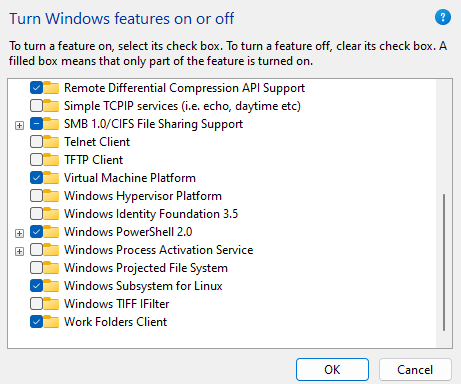
\includegraphics[width=0.65\textwidth]{images/wf}
	\caption{Windows Features.}
	\label{fig:wf}
\end{figure}
Now is is possible to install different subsystems. Open the command window - cmd.exe - and type
\begin{verbatim}
	wsl --list --online
\end{verbatim}
to get a list of the available OS-LST (Fig. \ref{fig:wsllist}).
\begin{figure}[ht]
	\centering
	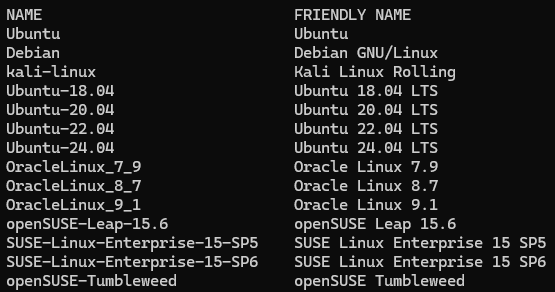
\includegraphics[width=0.65\textwidth]{images/wsllist}
	\caption{Available LTS systems.}
	\label{fig:wsllist}
\end{figure}
After having chosen the needed distribution, it is possible to install it. type
\begin{verbatim}
	wsl --install --OS_NAME
\end{verbatim}
to run the installation process. If instead it is typed just
\begin{verbatim}
	wsl --install
\end{verbatim}
the latest version of Ubuntu will be installed automatically. After the successful installation it will be required to insert a UNIX username and password. Once they are set, the installation will be completed (Fig. \ref{fig:is}).
\begin{figure}[ht]
	\centering
	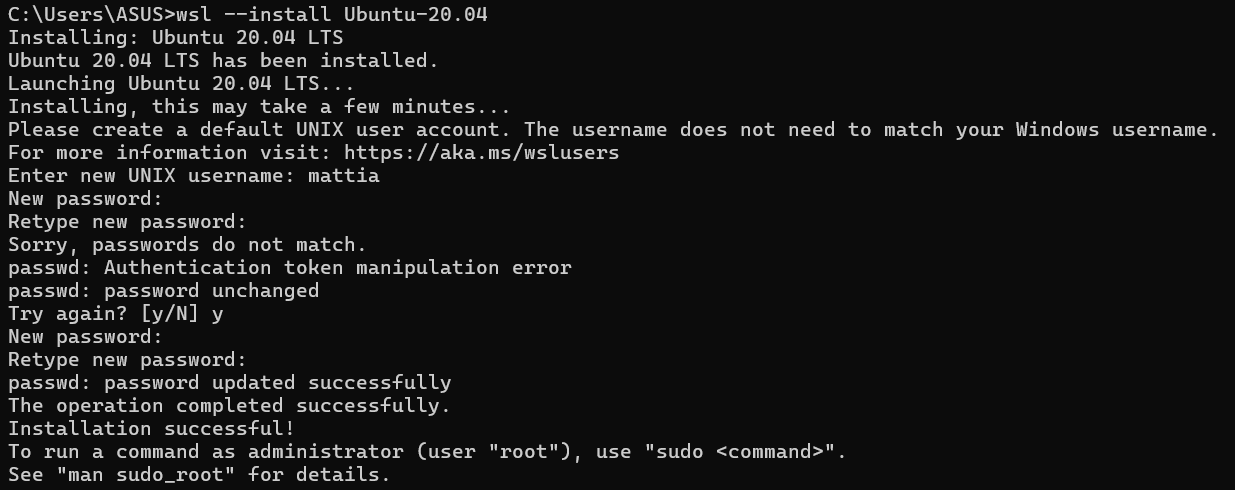
\includegraphics[width=0.65\textwidth]{images/is}
	\caption{Successful installation of the OS.}
	\label{fig:is}
\end{figure}
To use the terminal of the installed OS open the command prompt of windows, click on the down arrow on the top-left corner, near the "+" sign and choose the shell to be used (Fig. \ref{fig:fcmd}).
\begin{figure}[ht]
	\centering
	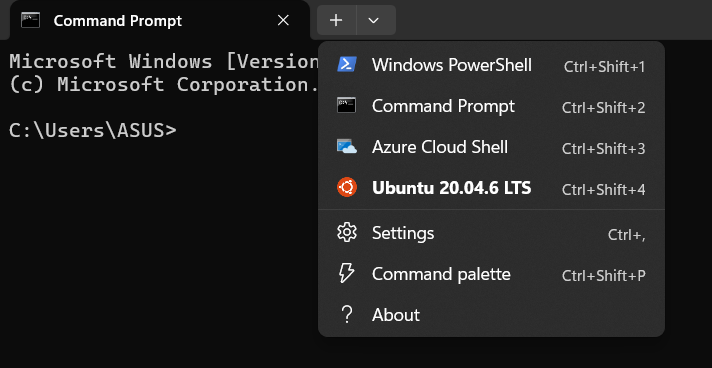
\includegraphics[width=0.65\textwidth]{images/fcmd}
	\caption{Using the shell.}
	\label{fig:fcmd}
\end{figure}
A new shell will pop-up and it is now possible to navigate just as if it was a machine running the chosen operating system. To check the correct version of Ubuntu type
\begin{verbatim}
	lsb_release -a
\end{verbatim}
and the OS data will be displayed in the prompt window.
\begin{figure}[ht]
	\centering
	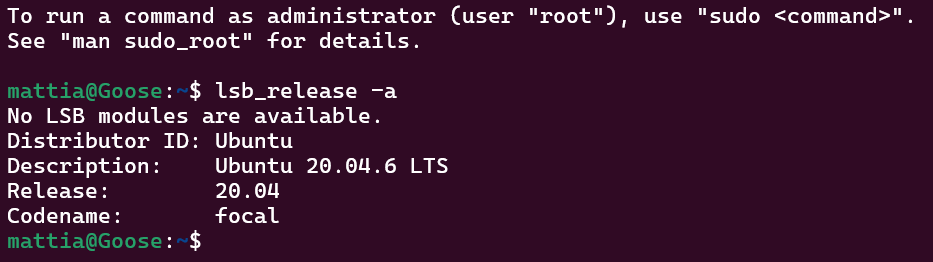
\includegraphics[width=0.65\textwidth]{images/ubshell}
	\caption{Ubuntu shell.}
	\label{fig:ubshell}
\end{figure}
If the Ubuntu version doesn't appear on the list of Fig. \ref{fig:fcmd}, restart the terminal.